\documentclass[12pt]{article}
\usepackage{graphicx}
\usepackage{fullpage}
\usepackage{verbatim}
\usepackage{caption}
\usepackage{float}
\usepackage[nottoc]{tocbibind} 
\usepackage{appendix}
\usepackage{titlesec}
\usepackage{tikz}
\usepackage{listings}
\usepackage{hyperref}
\hypersetup{
    colorlinks=true,
    linkcolor=blue,
    filecolor=magenta,      
    urlcolor=blue,
}
\usepackage[utf8]{inputenc}
\urlstyle{same}
\usetikzlibrary{shapes,arrows}
\titleformat{\chapter}[display]
  {\normalfont\bfseries}{}{0pt}{\Large}
  \usepackage[T1]{fontenc}
\usepackage[utf8]{inputenc}

  


\begin{document}
  \begin{titlepage}
    \begin{center}
      \begin{Large}
      \textbf{ Assignment- 11\\
       \vspace*{0.5cm}
       ELP - 718 Telecom Software Laboratory\\
       \vspace{1cm}
       Ch Krishna Chaitanya\\
       2019JTM2674\\
       2019-21\\}
      \end{Large}
       \vspace{1cm}
      {\Large  A report on Python with Kivy}
       \vfill
       \begin{figure}[h!]
          \centering
          
\includegraphics{iitdelhi.png}
       \end{figure}
       \vfill
      \begin{Large}
      \textbf{ Bharti School of \\
       Telecommunication Technology and Management\\
       IIT Delhi\\
       India\\
      }\end{Large}
       \medskip
       \today
    \end{center}
    \vfill
  \end{titlepage}
  
  \tableofcontents
  
  \clearpage
  \section*{Objective Statement}
   To test our understanding on implementation of kivy using python and to develop a application fror bank account management

  \section{Problem Statement -1}
 To design a Application for bank where user can create account, check balance, check last transactions, change password. Employee can update details of particular bank.
  
  \subsection{Algorithm and Implementation}
  \begin{itemize}
  \item Create static screens for user, employee login 
  \item Create database and tables as required
  \item Customer screen should validate password and also have provision for changing password
  \item Customer should be able to create a new account, delete account, check balance and money transfer
  \item Employee once logged in can modify user details
  \item Employee should be able to see bank details of customers
  \item Password validation is done using randomply generated OTP
  \item Respective Popups should be displayed when customer performs certain tasks.
  \end{itemize}
  \newpage
  \subsection{Flowchart}
    % Define block styles
\tikzstyle{decision} = [diamond, draw, fill=blue!20, 
    text width=4.5em, text badly centered, node distance=3cm, inner sep=0pt]
\tikzstyle{block} = [rectangle, draw, fill=blue!20, 
    text width=6.5em, text centered, rounded corners, minimum height=3em]
\tikzstyle{line} = [draw, -latex']
\tikzstyle{cloud} = [draw, ellipse,fill=red!20, node distance=3cm,
    minimum height=3em]
\begin{center}    
\begin{tikzpicture}[node distance = 2cm, auto]
    % Place nodes
    
    \node [cloud] (init) {start};
    \node [block, below of=init] (First) {Home Screen};
    \node [block, below of=First] (Second) {Select 1.Employee 2.Customer};
    \node [decision, below of=Second,node distance=3cm] (Third) {If Customer?};
     \node [decision, below of=Third,node distance=4cm] (Fouth) {Select 1.Login 2.Create Account};
     \node [block, left of=Third,node distance=5cm] (Fifth) {Enter User Id and Password};
     
    \node [block, below of=Fifth,node distance=2cm] (Sixth) {Modify Details};
    \node [block, below of=Fouth,node distance=3cm] (Seventh) {Enter Username and Password};
    \node [block, below of=Fifth,node distance=4cm] (Eigth) {Check Account Details};
    \node [cloud, below of=Eigth] (last_2) {stop};
    \node [block, below of=Fouth,node distance=6.5cm] (Ninth) {Select 1.Delete Account 2.Check Balance 3.Last Five Transactions 4.Transfer Money};
    \node [cloud, below of=Ninth] (last_1) {stop};
  \node [block, right of=Fouth,node distance=6.5cm] (Tenth) {Enter details};
   \node [block, below of=Tenth,node distance=4cm] (eleventh) {Account created};
    % Draw edges
    \path [line] (init) -- (First);
    \path [line] (First) -- (Second);
    \path [line] (Second) -- (Third);
     \path [line] (Third) -- node {Customer}(Fouth);
     \path [line] (Fouth) -- node {Login}(Seventh);
     \path [line] (Fouth) --node{Create Account}(Tenth);
     \path [line] (Third) -- node{Employee}(Fifth);
     \path [line] (Fifth) --(Sixth);
     \path [line] (Sixth) --(Eigth);
     \path [line] (Seventh) --(Ninth);
     \path [line] (Eigth) --(last_2);
     \path [line] (Tenth) --(eleventh);
     \path [line] (eleventh) |-(last_1);
      \path [line] (Ninth) --(last_1);
     
     
    
   
\end{tikzpicture}
\end{center}
  
 \newpage
  \subsection{Test Cases}
  
	\subsubsection{Input}
	Enter\\
1.Employee\\
2.Customer\\
\subsubsection{Output}
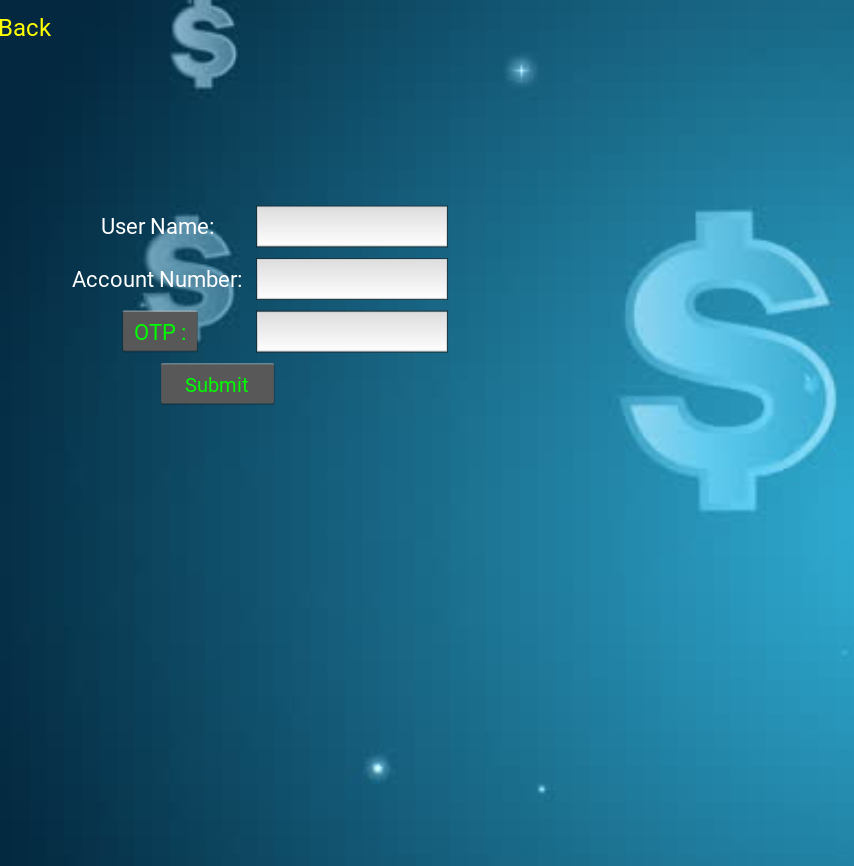
\includegraphics[width=\linewidth]{Lab_5.png}
\subsection{Screenshots}
\subsubsection{Screenshot1}

\includegraphics[width=\linewidth]{lab11_1.png}
\subsubsection{Screenshot2}
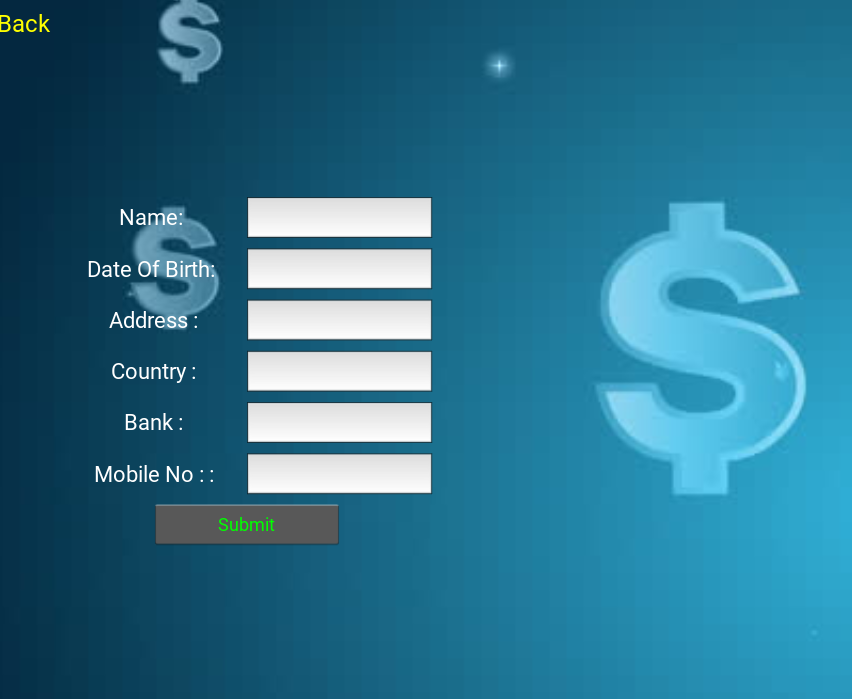
\includegraphics[width=\linewidth]{lab11_2.png}
\subsubsection{Screenshot2}
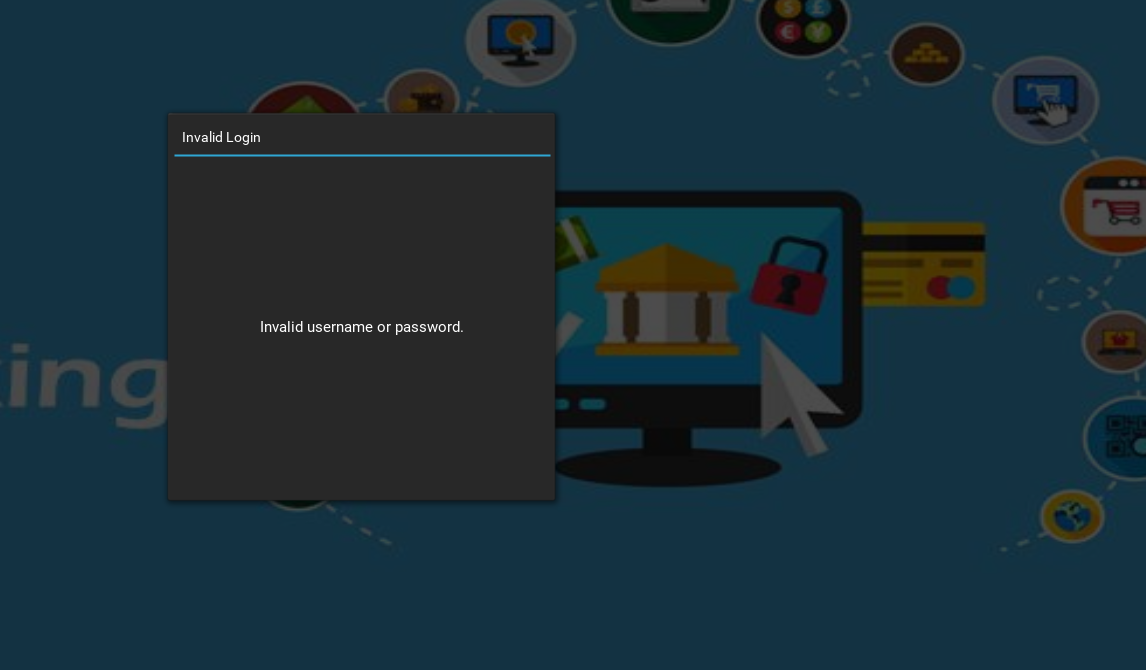
\includegraphics[width=\linewidth]{lab11_3.png}
\newpage
 \appendix
   \appendixpage
   \addappheadtotoc
  \section*{Problem 1}
  \subsection*{Python Code}
  {\large \textbf{code:}}
  \verbatiminput{ps1.py}
  \subsection*{Kivy Code}
  {\large \textbf{code:}}
  \verbatiminput{my.kv}
  
\newpage
\begin{thebibliography}{11}
\bibitem{flowchart} 
Flowchart using Latex\\
Kjell Magne Fauske \\
\url{http://www.texample.net/tikz/examples/simple-flow-chart/}

\bibitem{Python Basics}
Python Basics \\
\url{https://docs.python.org/3/}

\bibitem{SQL}
SQL\\
\url{https://www.w3schools.com/sql/sql_groupby.asp}

\bibitem{PyMySQl}
PyMySQl\\
\url{http://zetcode.com/python/pymysql/}

\bibitem{MySQL using Python}
MySQL using Python\\
\url{https://www.w3schools.com/python/python_mysql_select.asp}

\bibitem{Kivy using Python}
Kivy using Python\\
\url{https://techwithtim.net/tutorials/kivy-tutorial}

\bibitem{Kivy}
Kivy\\
\url{https://kivy.org/doc/stable/guide/basic.html}

\end{thebibliography}

   
   
\end{document}
